\documentclass{article}
\usepackage{import}
\usepackage{amsmath}
\usepackage{setspace}

\subimport*{./}{macro}
\setlength\parindent{0px}

\begin{document}
\title{Homework \#3}
\author{
    \normalsize{CSE 446/546: Machine Learning}\\
    \normalsize{Zuo Wang}\\
}
\date{{}}
\maketitle


% Quesetion 1
\begin{spacing}{3}{\bfseries\LARGE Question 1}\end{spacing}
\textbf{(a.)}
\begin{flushleft}
    We should decrease $\sigma$ because decreasing the bandwith allows us to have a more localized and complex model.
    Mathmatically speaking, decreasing $\sigma$ makes the kernel value smaller (exponential of a larger negative value)
    therefore the penalty term is smaller, resulting in a more complex model.
\end{flushleft}

\vspace{5mm}\textbf{(b.)}
\begin{flushleft}
    False. Most neural networks actually have non-convex loss functions.
\end{flushleft}

\vspace{5mm}\textbf{(c.)}
\begin{flushleft}
    False. If we initialize all weights to zero when training a deep neural network, the gradient of all the weights will
    be the same during backpropagation, resulting in all neurons learning the same features and updating their weights identically.
\end{flushleft}

\vspace{5mm}\textbf{(d.)}
\begin{flushleft}
    True. Linear activation functions would result in a network that can only learn linear decision boundaries.
\end{flushleft}

\vspace{5mm}\textbf{(e.)}
\begin{flushleft}
    True. The backward pass step requires computing the gradients of the loss with respect to the parameters, 
    which involves matrix multiplications, and derivating activation function. And that is more time-consuming compared to the forward pass step.
\end{flushleft}

\vspace{5mm}\textbf{(f.)}
\begin{flushleft}
    False. While neural network is consider one of the best models in most cases, it is not always the best choice for every circumstance.
    Generally speaking, neural networks are more complex, require a longer runtime, are better for larger dataset, and tend to overfit. 
    In some cases, simple models with regularization might just perform better.
\end{flushleft}


% Quesetion 2
\pagebreak
\begin{spacing}{3}{\bfseries\LARGE Question 2}\end{spacing}
\textbf{(a.)}

\vspace{5mm}\textbf{(b.)}
\begin{flushleft}
    From the support vectors and their corresponding labels, we know that:
\end{flushleft}
\begin{center}
    $\begin{bmatrix}1 \\ 2 \\\end{bmatrix} w + b = -1$,
    $\begin{bmatrix}0 \\ 0.5 \\\end{bmatrix} w + b = 1$,
    $\begin{bmatrix}2 \\ 1 \\\end{bmatrix} w + b = 1$
\end{center}
Looking at the last two equations, we can construct the matrix:
\begin{align*}
    w &= \left[\begin{array}{@{}cc|c@{}}
        0 & 0.5 & 1-b \\
        2 & 1 & 1-b
    \end{array}\right]
    \\&= \left[\begin{array}{@{}cc|c@{}}
        2 & 1 & (1-b) \\
        0 & 1 & 2(1-b)
    \end{array}\right]
    \\&= \left[\begin{array}{@{}cc|c@{}}
        1 & 0 & -\frac{1}{2}(1-b) \\
        0 & 1 & 2(1-b)
    \end{array}\right]
    \\&= \left[-\frac{1}{2}(1-b) \;\;\;\; 2(1-b)\right]
\end{align*}
And we plug $w$ back into $\begin{bmatrix}1 \\ 2 \\\end{bmatrix} w + b = -1$:
\begin{align*}
    \begin{bmatrix}1 \\ 2 \\\end{bmatrix} \cdot \left[-\frac{1}{2}(1-b) \;\;\;\; 2(1-b)\right] + b &= -1
    \\ -\frac{1}{2}(1-b) + 4(1-b) + b &= -1
    \\ \frac{7}{2}(1-b) + b &= -1
    \\ -\frac{5}{2} b &= -\frac{9}{2}
    \\ b &= \frac{9}{5}
\end{align*}
\begin{center}
    \boxed{
    b = \frac{9}{5} \;\;
    w = \left[\frac{2}{5} \;\;\;\; -\frac{8}{5}\right]}
\end{center}

\vspace{5mm}\textbf{(c.)}


% Quesetion 3
\pagebreak
\begin{spacing}{3}{\bfseries\LARGE Question 3}\end{spacing}
\begin{align*}
    \phi (x) \cdot \phi (x') &= \sum_{i=0}^{\infty}
    \left( \frac{1}{\sqrt{i!}} e^{\frac{-x^2}{2}}x^i \right) \cdot 
    \left( \frac{1}{\sqrt{i!}} e^{\frac{-x'^2}{2}}(x')^i \right)
    \\&= \sum_{i=0}^{\infty} \frac{1}{i!} e^{\frac{-(x^2+x'^2)}{2}} x^i(x')^i
    \\&= e^{\frac{-(x^2+x'^2)}{2}}
    \sum_{i=0}^{\infty} \frac{1}{i!} x^i(x')^i
\end{align*}
Because the Taylor expansion of $e^z = \sum_{n=0}^{\infty} \frac{1}{n!}z^n$, 
the summation above just becomes $e^{xx'}$, therefore:
\begin{align*}
    \phi (x) \cdot \phi (x') &= e^{\frac{-(x^2+x'^2)}{2}} \cdot e^{xx'}
    \\&= e^{\frac{-x^2 -x'^2 + 2xx'}{2}}
    \\&= e^{\frac{-(x - x')^2}{2}}
\end{align*}

% Quesetion 4
\pagebreak
\begin{spacing}{4}{\bfseries\LARGE Question 4}\end{spacing}
\textbf{(a.)}
\begin{flushleft}
    For the RBF kernel, $\lambda_{optimal} = 10^{-3}$, $\;\gamma_{optimal} = 10.5416$\\
    For the polynomial kernel, $\lambda_{optimal} = 10^{-3}$, $\;d_{optimal} = 20.5102$
\end{flushleft}

\vspace{5mm}\textbf{(b.)}
\begin{center}
    $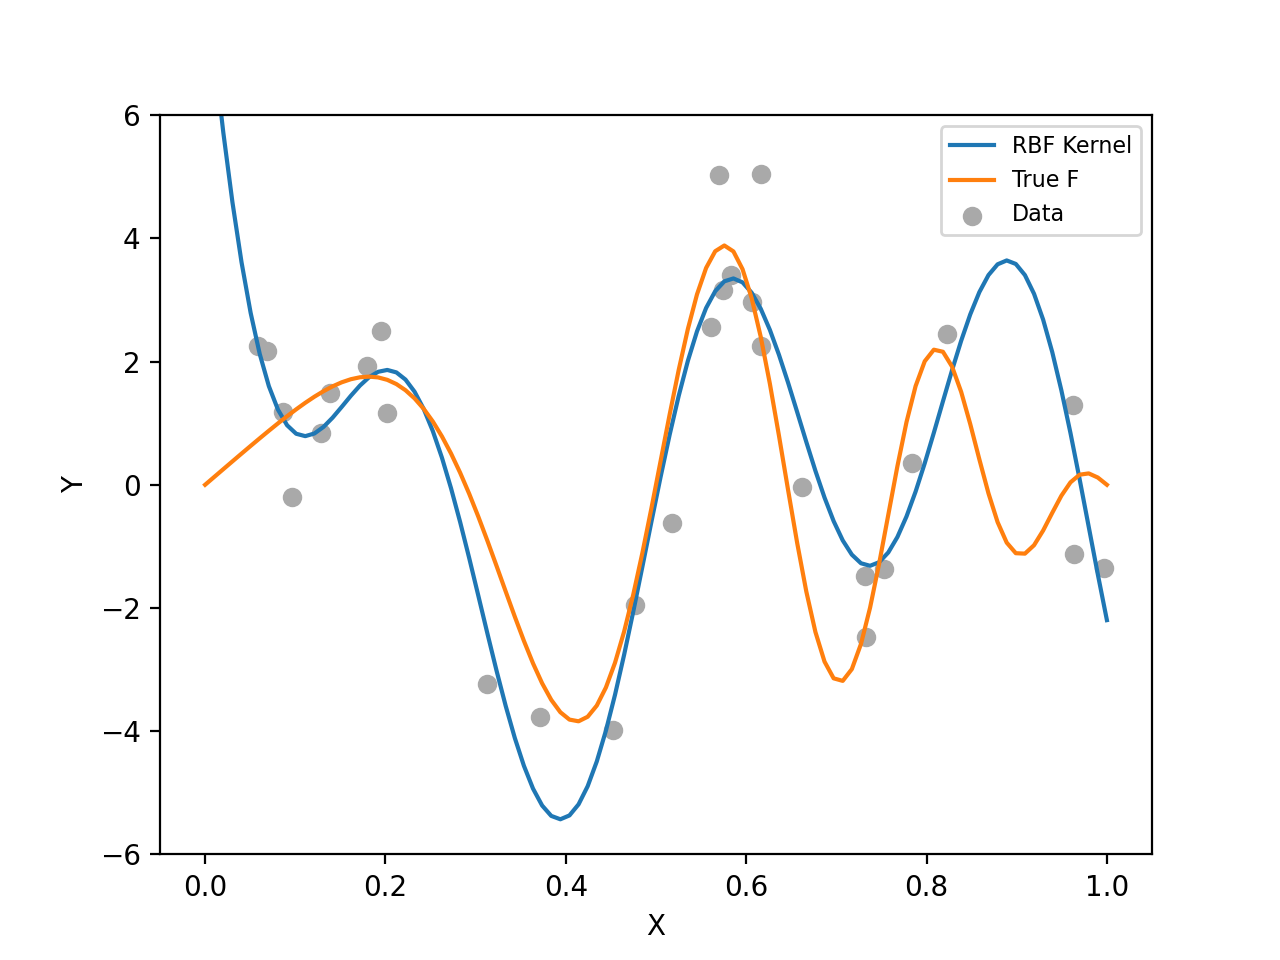
\includegraphics[width=0.7\textwidth] {/Users/zuo/Desktop/School/SP 23/CSE 446/hw3/figures/a4_rbf.png}$
    $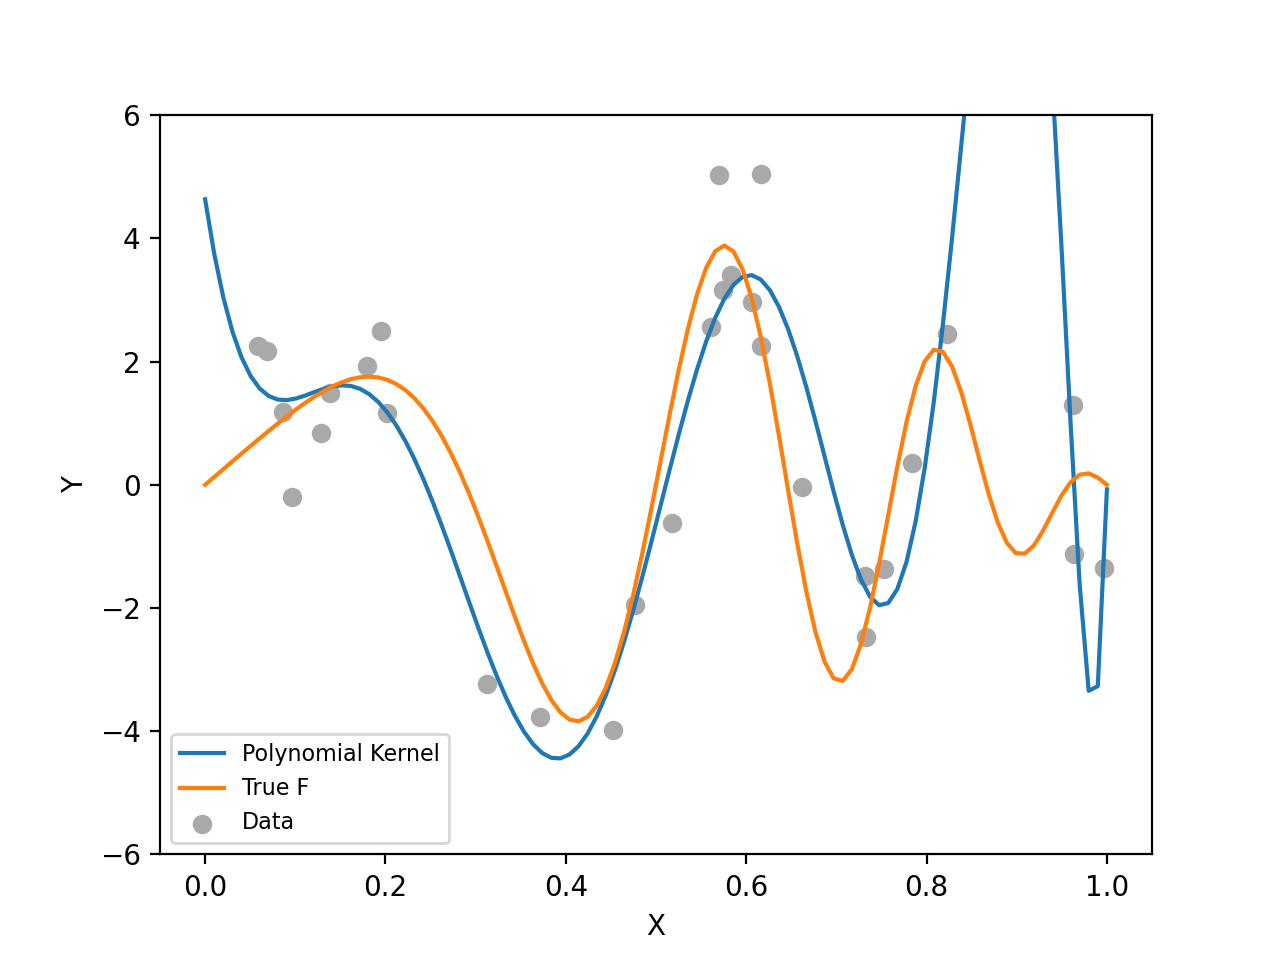
\includegraphics[width=0.7\textwidth] {/Users/zuo/Desktop/School/SP 23/CSE 446/hw3/figures/a4_poly.png}$
\end{center}



% Quesetion 5
\pagebreak
\begin{spacing}{3}{\bfseries\LARGE Question 5}\end{spacing}


% Quesetion 6
\pagebreak
\begin{spacing}{3}{\bfseries\LARGE Question 6}\end{spacing}

\end{document}